Wide ResNet achieves an accuracy of 86.3\%  which is much higher than the state-of-the-art accuracy on the FER+ dataset. Also we observe that the top-2 accuracy is 95.69\%, and the top-3 accuracy is 98.35\% which are both very high. So the idea is to create an additional model that will give an extra "opinion" about the predicted emotion when our main network (Wide ResNet) has no clear winner (when the probabilities of the top labels are close to each other). To create a new model that will provide an extra assistance to our main model we use action units which encode facial muscle movement. More concretely, we use OpenFace~\cite{baltruvsaitis2016openface}, an open source tool capable of facial landmark detection, head pose estimation, facial action unit recognition, and eye-gaze estimation. By using this tool we can create a separate dataset with action units to serve as the features and the emotions to be the labels. The next step is to train an SVM classifier for every pair of emotions. We only take as features, the action units that are associated with the two emotions of the binary classification as depicted in table~\ref{tab:AU}. Also we train an SVM classifier for every 3 emotions. By using these two extra models we increase the accuracy from 86.3\% to 86.6\%. The algorithm is depicted in Figure~\ref{fig:final_model}.

 \begin{figure}[]
    \begin{center}
    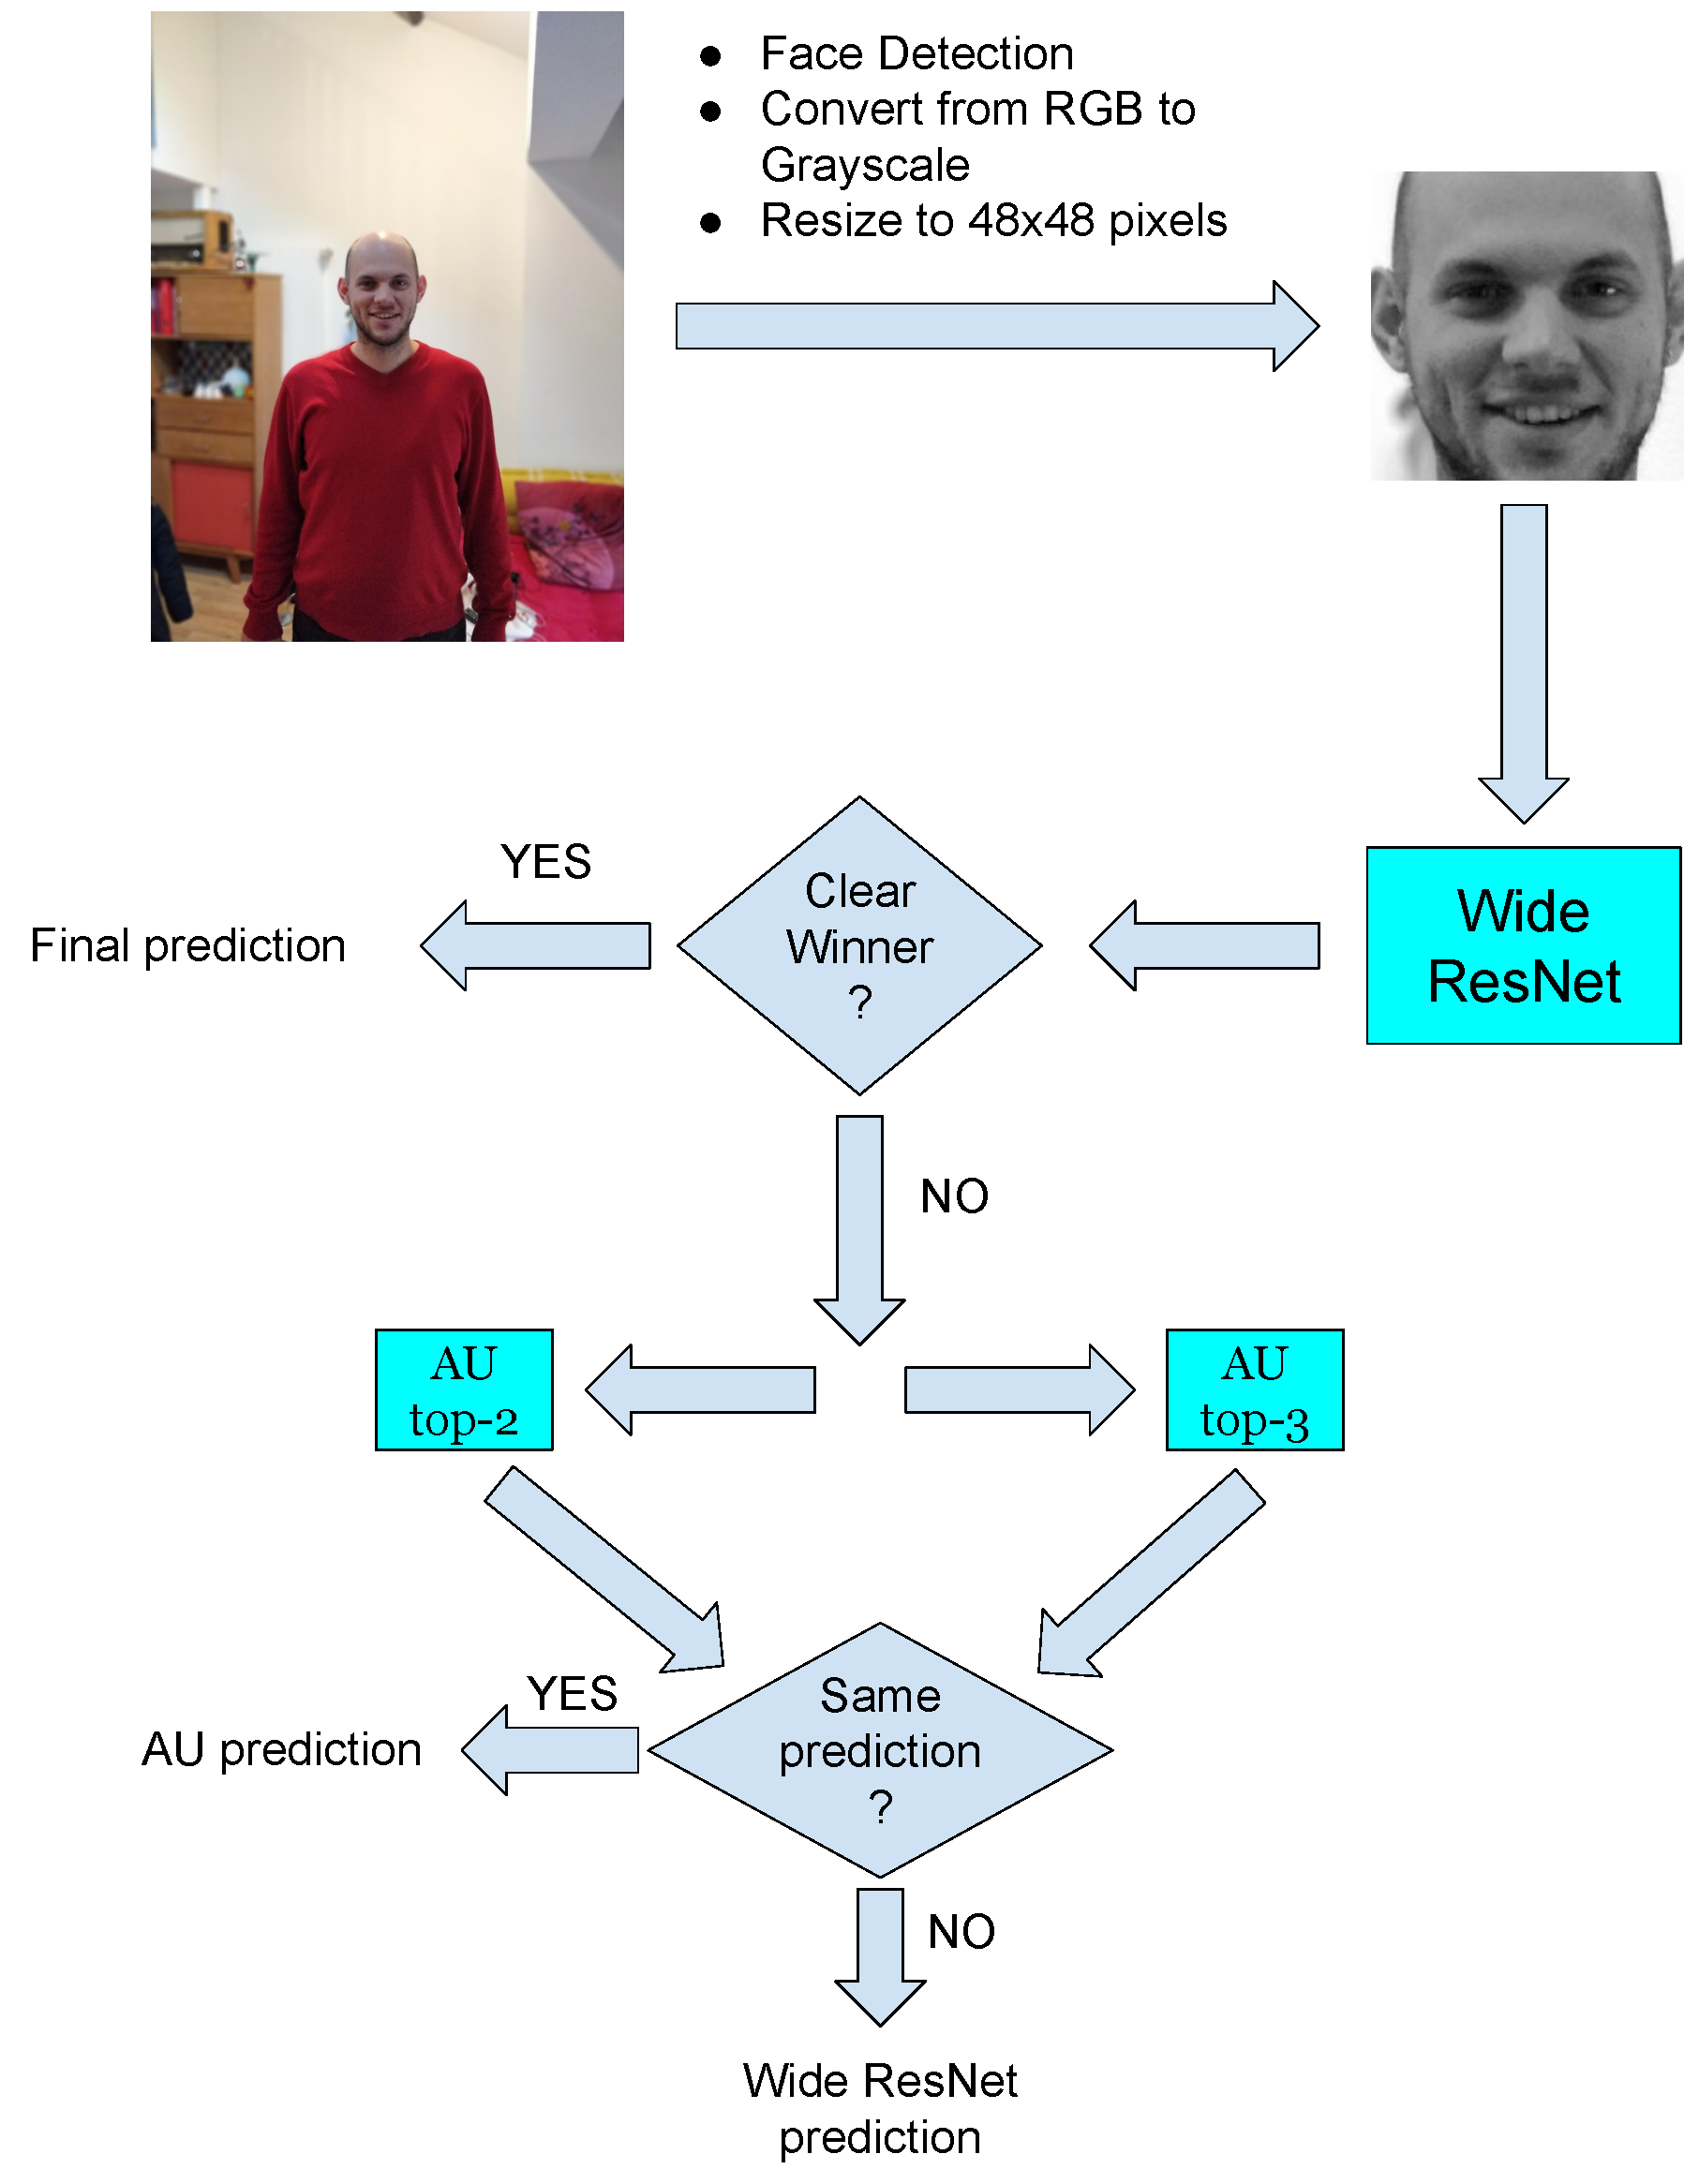
\includegraphics[width=1.0\textwidth]{images/final_model.pdf}
    \end{center}
    \caption{Final Algorithm.} \label{fig:final_model}
\end{figure}